\documentclass[10pt]{article}

% -----------------------------------------------------------------------------
% Page and typography (kept from the supplied version)
% -----------------------------------------------------------------------------
\usepackage[letterpaper,margin=1.1in]{geometry}
\usepackage[T1]{fontenc}
\usepackage{lmodern}
\usepackage{microtype}
\usepackage{graphicx}
\usepackage{booktabs}
\usepackage{array}
\usepackage{amsmath}
\usepackage{xcolor}
\usepackage{enumitem}
\usepackage{caption}
\usepackage{tikz}
\usetikzlibrary{arrows.meta,positioning}
\usepackage[hidelinks]{hyperref}
\usepackage{url}
\usepackage{float}
\usepackage{siunitx}

\graphicspath{{figures/}}
\setlength{\parindent}{0pt}
\setlength{\parskip}{2.2pt}
\setlength{\textfloatsep}{4pt}
\setlength{\floatsep}{3pt}
\setlength{\intextsep}{3pt}
\captionsetup{font=footnotesize,skip=2pt}
\setlist[itemize]{leftmargin=1.2em,itemsep=0pt,topsep=1pt}
\setlist[enumerate]{leftmargin=1.3em,itemsep=0pt,topsep=1pt}
\renewcommand{\arraystretch}{1.03}

% -----------------------------------------------------------------------------
% Custom macros
% -----------------------------------------------------------------------------
\newcommand{\sysquestion}{Under the same model, dataset, precision, and training-token budget, can LoRA reduce memory and storage, increase throughput and feasible micro-batch size, and preserve GSM8K quality?}

\begin{document}
\small

\begin{center}
{\Large\bfseries LoRA vs. Full Fine-Tuning for Reasoning:\ A Single-GPU Systems Study}\\[1mm]
{\normalsize Daoyuan Guo \qquad Zhaokai Liang}\\[-1mm]
{\footnotesize ML Systems, Summer 2026}
\end{center}
\vspace{-2mm}

% =============================================================================
% FOUR-PAGE MAIN BODY BEGINS
% =============================================================================
\section*{1. Problem and System Overview}

Full fine-tuning (Full FT) updates all model weights and therefore stores gradients and AdamW optimizer state for the full model. LoRA freezes the pretrained weights and learns low-rank updates, reducing trainable state and task-specific storage~\cite{hu2022lora}. Our systems question is: \emph{\sysquestion}

We implement an end-to-end training-to-evaluation slice for Qwen3.5-0.8B on GSM8K~\cite{cobbe2021gsm8k}. The system formats and tokenizes examples, trains either Full FT or LoRA-r16 in BF16 on one NVIDIA A40, exports a full checkpoint or adapter, performs offline greedy inference, and computes exact match. Online serving is not implemented; serving is optional for this archetype, so we prioritize a deeper single-GPU training study with a measured path from data preparation to a reusable model artifact and task-quality evaluation.

The project is a systems study rather than only a model comparison. Fewer trainable parameters are useful only if they reduce the total device footprint or permit a better operating point. We therefore treat peak allocated memory, non-padding tokens/s, maximum feasible micro-batch, training time, and artifact size as first-class outputs, and use GSM8K exact match to check whether the systems savings come with an evident quality loss.

\begin{figure}[H]
\centering
\resizebox{0.98\linewidth}{!}{%
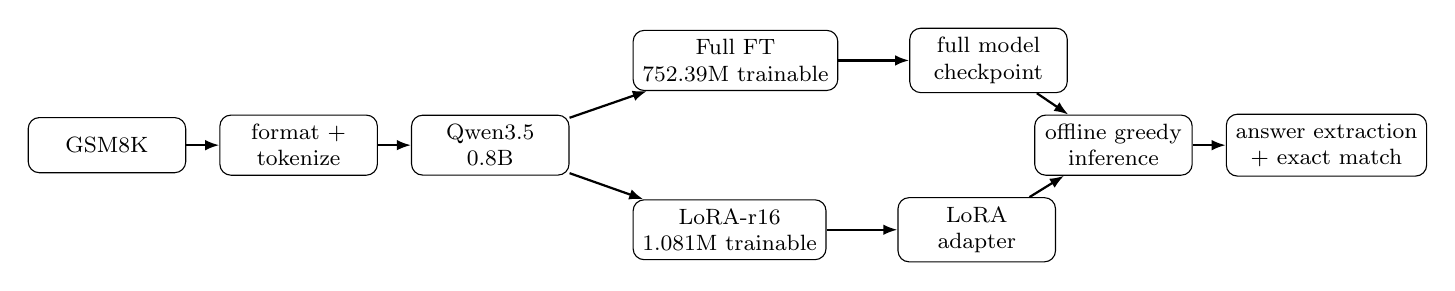
\begin{tikzpicture}[
node distance=4.2mm,
box/.style={draw,rounded corners,align=center,minimum height=7mm,minimum width=20mm,font=\footnotesize},
arrow/.style={-{Latex[length=1.8mm]},thick}]
\node[box] (data) {GSM8K};
\node[box,right=of data] (prep) {format +\\tokenize};
\node[box,right=of prep] (model) {Qwen3.5\\0.8B};
\node[box,above right=3mm and 8mm of model] (full) {Full FT\\752.39M trainable};
\node[box,below right=3mm and 8mm of model] (lora) {LoRA-r16\\1.081M trainable};
\node[box,right=9mm of full] (fart) {full model\\checkpoint};
\node[box,right=9mm of lora] (lart) {LoRA\\adapter};
\node[box,right=12mm of model,xshift=47mm] (infer) {offline greedy\\inference};
\node[box,right=of infer] (score) {answer extraction\\+ exact match};
\draw[arrow] (data)--(prep); \draw[arrow] (prep)--(model);
\draw[arrow] (model)--(full); \draw[arrow] (model)--(lora);
\draw[arrow] (full)--(fart); \draw[arrow] (lora)--(lart);
\draw[arrow] (fart)--(infer); \draw[arrow] (lart)--(infer); \draw[arrow] (infer)--(score);
\end{tikzpicture}}
\caption{Implemented slice. Full FT exports a complete task model, whereas LoRA exports an adapter used with the shared base model.}
\label{fig:pipeline}
\end{figure}

\section*{2. Design}

\textbf{Adaptation flexibility vs. systems efficiency.} Full FT permits unrestricted weight updates but pays for gradients, two AdamW moment tensors, and a full task checkpoint. LoRA represents each adapted matrix as $W'=W+BA$, where $r\ll d$, trading update flexibility for a much smaller trainable state. Base weights, activations, kernels, and temporary buffers remain; therefore a $696\times$ reduction in trainable parameters need not become a $696\times$ reduction in total GPU memory. This distinction is central to our evaluation: parameter count predicts a direction, while the measured peak captures the complete training process.

\textbf{Memory-budget reasoning.} In BF16, the 752.39M base parameters alone require roughly 1.50~GB. Full FT additionally needs same-scale gradients and substantially larger FP32 AdamW moment state, before accounting for activations and temporary workspaces. LoRA retains the base-weight cost but allocates gradients and optimizer state only for 1.081M adapter parameters. We therefore expect a large but bounded memory gap, with the relative advantage shrinking as activation memory grows at larger micro-batches or sequence lengths.

\textbf{Use saved memory as batch capacity.} We fix effective batch size 16 and approximately one million non-padding training tokens, then sweep micro-batch $\{1,2,4,8,16\}$ while adjusting gradient accumulation. This tests whether lower optimizer-state memory creates a practical gain rather than only a smaller parameter count. Larger micro-batches expose more parallel work but increase activation memory, so the largest feasible batch may not be the fastest. The resulting curve identifies both the OOM boundary and the batching knee.

\textbf{Equal tuning budget, not an identical learning rate.} Full FT and LoRA optimize different parameterizations and gradient scales. We therefore tune both with the same AdamW grid $\{2\!\times\!10^{-5},5\!\times\!10^{-5},10^{-4},2\!\times\!10^{-4}\}$, the same three selection seeds, the same validation split, and the same token budget. Mean validation first-turn exact match selects $2\times10^{-5}$ for Full FT and $2\times10^{-4}$ for LoRA-r16. The official test set is used only after these rates are fixed. The measured sweep shows that this is not merely procedural hygiene: the two methods respond to the learning rate in \emph{opposite} directions, so a single shared rate would have decided the outcome of the study before any systems measurement was taken. At $2\times10^{-5}$ the two methods are statistically indistinguishable (39.9\% vs.\ 39.7\%), whereas at $2\times10^{-4}$ they differ by 45 points because Full FT has collapsed. Reporting either shared-rate comparison would have been defensible in form and misleading in substance. The design removes the criticism that one method was granted a more suitable learning rate while acknowledging that the finite grid does not prove global optimality.

\textbf{Measurement and scope choices.} We use peak \emph{allocated} CUDA memory rather than reserved memory because the latter depends strongly on PyTorch's caching allocator. Throughput counts non-padding training tokens, avoiding an artificial gain from padding. We repeat the final operating point over five seeds and keep the rank and sequence-length experiments as single-seed ablations. We deliberately omit an online endpoint, p95/p99 serving latency, llama.cpp deployment, and multi-GPU scaling: depth on the training-memory trade-off is more valuable here than a broader but weakly measured feature list.

\section*{3. Implementation}

The runnable slice is configuration-driven. A data loader creates deterministic GSM8K train/validation/test inputs, applies the same prompt template to both methods, and reports non-padding token counts. The model factory loads Qwen3.5-0.8B and either exposes all parameters for Full FT or inserts rank-16 LoRA modules into the query, key, value, and output attention projections. Both paths use BF16, AdamW~\cite{loshchilov2019adamw}, gradient accumulation, and the same token-budget stopping rule.

The training runner resolves each YAML configuration, sets the random seed, resets CUDA peak statistics after initialization, and records peak allocated memory, wall-clock time, optimizer steps, non-padding tokens/s, trainable parameters, artifact size, and failures. Each successful run writes its resolved configuration, metadata, metrics, and task artifact. OOM is retained as a measured outcome rather than discarded, because the feasibility boundary directly answers the batch-capacity question.

Evaluation performs deterministic greedy generation and writes one JSONL record per scored example, including the raw generated text, extracted answer, gold answer, and correctness. Which split is scored is part of the configuration: tuning configurations score the 500-example validation split, and every reported configuration scores the official test split, so the selection stage cannot silently consume test data. Each record and each run report both answer-extraction rules described in Section~4, and each run also records the mean validation loss used as the selection tie-breaker. The submitted implementation is real from data loading through offline inference. Online request handling, p95/p99 serving latency, llama.cpp deployment, and multi-GPU execution are not implemented. The artifact README should reproduce the headline numbers from a clean source revision and include exact commands, resolved configurations, environment versions, raw predictions, and failure records.

\section*{4. Evaluation}

\textbf{Setup and protocol.} Experiments use one NVIDIA A40, Qwen3.5-0.8B, GSM8K, BF16, maximum length 512, micro-batch 2, effective batch 16, and approximately one million non-padding training tokens for the main comparison. Final results use seeds 11, 22, 33, 44, and 55. The GPU is checked for unrelated processes before timing; model construction and initial warm-up are excluded from the training interval. The named baseline is tuned Full FT at $2\times10^{-5}$, while LoRA-r16 uses its independently selected $2\times10^{-4}$.

\textbf{Learning-rate control.} Both methods receive the same four-rate grid and three-seed validation budget, for 24 tuning runs in total. Table~\ref{tab:lrsummary} summarizes the completed selection sweep; the complete protocol is in Appendix~\ref{app:lr}. The selected rates are $2\times10^{-5}$ for Full FT and $2\times10^{-4}$ for LoRA-r16. Both rows are monotone and they point in opposite directions: Full FT loses 97\% of its accuracy across the grid (39.9\% to 1.1\%), while LoRA-r16 gains 17\% relative (39.7\% to 46.5\%). Mean validation loss orders the cells identically in both rows, so the documented tie-breaker was never needed. Full FT is therefore not merely sensitive to the learning rate; outside a narrow band it stops solving the task at all, which is exactly the failure a shared-rate comparison would have hidden. This supports a comparison of equally tuned methods rather than an identical-rate ablation.

\begin{table}[H]
\centering
\caption{Common-grid validation sweep. Mean validation first-turn exact match ($\%$) $\pm$ standard deviation over selection seeds 11, 22, and 33.}
\label{tab:lrsummary}
\begin{tabular}{lcccc}
\toprule
& $2\times10^{-5}$ & $5\times10^{-5}$ & $10^{-4}$ & $2\times10^{-4}$ \\
\midrule
Full FT & $\mathbf{39.9 \pm 2.2}$ & $21.5 \pm 3.1$ & $6.6 \pm 1.4$ & $1.1 \pm 0.4$ \\
LoRA-r16 & $39.7 \pm 2.4$ & $43.5 \pm 2.8$ & $45.9 \pm 0.6$ & $\mathbf{46.5 \pm 1.5}$ \\
\bottomrule
\end{tabular}
\end{table}

\textbf{Main operating point.} LoRA-r16 reduces peak allocated memory from $11.103\pm0.012$~GB to $6.170\pm0.005$~GB, a $44.4\%$ reduction. Throughput increases from $2169\pm22$ to $2384\pm18$ non-padding tokens/s, a $9.9\%$ gain, and mean training time falls by about $9.0\%$. Trainable parameters fall from 752.39M to 1.081M, while the task artifact shrinks from 1454.19~MB to 23.21~MB ($62.7\times$). The memory and throughput gaps are much larger than their seed-level variation, whereas corrected exact-match distributions overlap.

\begin{figure}[h]
\centering
\includegraphics[width=0.58\linewidth]{figure1_main_tradeoff.png}
\caption{Five-seed main comparison. LoRA-r16 lowers peak allocated memory and raises training throughput; quality is treated as comparable rather than ranked.}
\label{fig:maintradeoff}
\end{figure}

\textbf{Saved memory becomes useful batch capacity.} At micro-batch 8, LoRA-r16 reaches 6954 tokens/s versus 5309 tokens/s for Full FT, a $31.0\%$ gain, while using 20.18~GB instead of 27.28~GB, a $26.0\%$ reduction. Full FT OOMs at micro-batch 16, whereas LoRA completes at 38.91~GB. LoRA throughput falls slightly from micro-batch 8 to 16, revealing a batching knee: feasibility continues to increase after throughput saturates. This is the strongest operational consequence of the memory saving because it converts lower state cost into a workload that Full FT cannot execute on the same device.

\begin{figure}[h]
\centering
\includegraphics[width=0.72\linewidth]{figure2_batch_scaling.png}
\caption{Micro-batch sweep at maximum length 512 and effective batch 16. The largest feasible LoRA batch is not the highest-throughput point.}
\label{fig:batch}
\end{figure}

\textbf{Quality and parser sensitivity.} Full FT generations often continue after one answer and emit another role boundary or repeated final-answer marker. The original last-answer parser therefore lowers Full FT mean exact match to 33.57\%. Our primary rule stops at the first generated role boundary and grades the last complete answer in that assistant turn. Under this rule, five-seed exact match is $38.83\%$ for Full FT, $39.88\%$ for LoRA-r8, and $40.61\%$ for LoRA-r16. The quality distributions overlap, so the supported claim is ``no clear mean decrease,'' not LoRA superiority or formal equivalence. The tuning sweep localizes the effect precisely: a role boundary appears in $35.9\%$ of Full FT generations at $2\times10^{-5}$ and in $0.0\%$ of generations in every other cell of the grid, and the two rules therefore disagree only for Full FT at its selected rate ($39.9\%$ versus $36.8\%$) and agree to the digit everywhere else. Parser sensitivity is thus a property of a competent model that does not stop, not a general property of Full FT. It must not be confused with the distinct high-rate failure in which reasoning itself collapses and no answer-extraction rule can recover the score. Rescoring the stored text corrects answer extraction but cannot reproduce generations under a repaired EOS configuration because checkpoints and raw token IDs are unavailable.

\begin{figure}[h]
\centering
\includegraphics[width=0.69\linewidth]{figure6_quality_sensitivity.png}
\caption{Exact-match sensitivity to answer extraction on the same stored predictions. Full FT is parser-sensitive; LoRA is comparatively stable.}
\label{fig:quality}
\end{figure}

\textbf{Ablations and interpretation.} Raising LoRA rank from 4 to 32 increases adapter parameters by $8\times$ but peak memory by less than $1\%$ (6.154 to 6.201~GB). Throughput remains approximately flat, so the small non-monotonic differences are treated as run-to-run variation rather than a rank-speed law. Sequence length changes memory more than rank because longer padded batches increase activation state. Together, the results show that base-model computation and activations dominate the small LoRA-rank changes, while optimizer-state savings dominate the Full-FT comparison. The learning-rate sweep adds a third axis to this picture: LoRA's advantage at the main operating point is a systems advantage, but its tolerance of a $10\times$ larger learning rate is an optimization-side advantage that the memory and throughput measurements do not capture.

\textbf{Limitations.}
\begin{itemize}
    \item Results cover one model, dataset, precision, GPU, sequence distribution, and training-token budget; they do not establish a universal LoRA speedup.
    \item Learning-rate fairness is limited to the tested common grid, and both selected rates sit on a grid boundary. LoRA-r16 was still improving in both exact match and validation loss at the largest rate, and Full FT was best at the smallest rate, so each method's optimum may lie outside the tested range in opposite directions. The grid establishes that the two methods need different rates; it does not establish the best rate for either.
    \item Rank and sequence-length sweeps use one seed, while only the main operating point and quality comparison use five seeds.
    \item Validation and test numbers are not interchangeable. The validation split is carved from official train and is measurably easier: at the selected rates the same three seeds score 36.8\% on validation versus 35.0\% on test for Full FT, and 46.5\% versus 40.7\% for LoRA-r16 under the last-answer rule. Validation numbers are used for selection only.
    \item Stored predictions can be rescored, but missing checkpoints and raw token IDs prevent corrected-EOS regeneration.
    \item The archived runs originally recorded dirty source trees; the final artifact must pin a clean commit or include a complete source snapshot.
    \item The FlashAttention-labeled rerun lacks verified backend provenance and remains appendix-only rather than a causal result.
\end{itemize}

\section*{5. Individual-Contribution Statement}

Daoyuan Guo designed and implemented the whole training pipeline as well as experiments, and collected memory and throughput measurements. Zhaokai Liang implemented data processing and quality evaluation. Both members interpreted results, prepared artifacts, and revised the report and presentation.\\[-1mm]

\textit{Agreed by:} Daoyuan Guo, Zhaokai Liang

\section*{6. AI-Use Acknowledgment}

ChatGPT was used to brainstorm the learning-rate control, organize a LaTeX working draft, and assist with wording and formatting. It did not run the experiments or originate measurements. The authors verified all reported values against project artifacts, revised the final prose, and accept responsibility for every claim.

\begin{center}
\fbox{\parbox{0.94\linewidth}{\centering\footnotesize
\textbf{Supported conclusion.} For Qwen3.5-0.8B on GSM8K with BF16 on one A40, equally tuned LoRA-r16 is the stronger systems operating point: it uses less memory, trains faster, supports a larger micro-batch, and produces a much smaller task artifact without a clear mean decrease in corrected exact match.}}
\end{center}

% =============================================================================
% REFERENCES AND APPENDIX (excluded from the four-page main body)
% No forced page break is used; these begin after the main body naturally fills.
% =============================================================================
\begin{thebibliography}{8}\footnotesize
\bibitem{hu2022lora} E. J. Hu et al., ``LoRA: Low-Rank Adaptation of Large Language Models,'' \emph{ICLR}, 2022.
\bibitem{cobbe2021gsm8k} K. Cobbe et al., ``Training Verifiers to Solve Math Word Problems,'' arXiv:2110.14168, 2021.
\bibitem{loshchilov2019adamw} I. Loshchilov and F. Hutter, ``Decoupled Weight Decay Regularization,'' \emph{ICLR}, 2019.
\bibitem{pytorch} A. Paszke et al., ``PyTorch: An Imperative Style, High-Performance Deep Learning Library,'' \emph{NeurIPS}, 2019.
\bibitem{qwen} Qwen Team, ``Qwen3.5-0.8B model card,'' Hugging Face model repository, accessed July 2026.
\end{thebibliography}

\appendix
\newpage
\section{Learning-Rate Control}\label{app:lr}

The same fixed validation split and seeds 11, 22, and 33 are used for both methods, giving $2\times4\times3=24$ tuning runs. All configurations use BF16, micro-batch 2, effective batch 16, maximum length 512, the same warmup, weight decay, gradient clipping, data order, and approximately one million non-padding training tokens. Selection uses mean validation first-turn exact match, with validation loss as a tie-breaker; no cell tied, so the tie-breaker did not affect either selection. Tuning runs are scored on the 500 held-out validation examples and save no checkpoint, because a rate that is not selected has no artifact worth keeping. The official test set is untouched until the final five-seed comparison.

Validation loss agrees with exact match in both rows and in both directions, which makes the selection robust to the choice of selection metric: for Full FT the loss rises monotonically from 0.421 to 0.987 as the rate increases, and for LoRA-r16 it falls monotonically from 0.508 to 0.457. The two criteria would select the same rate for each method independently.

\begin{table}[H]
\centering
\caption{Complete learning-rate selection table. Bold entries are selected based on the sweep. Each entry is the mean over seeds 11, 22, and 33.}
\begin{tabular}{llcc}
\toprule
Method & AdamW learning rate & Validation first-turn EM ($\%$) & Validation loss \\
\midrule
Full FT & $2\times10^{-5}$ & $\mathbf{39.9 \pm 2.2}$ & $\mathbf{0.421}$ \\
Full FT & $5\times10^{-5}$ & $21.5 \pm 3.1$ & $0.508$ \\
Full FT & $1\times10^{-4}$ & $6.6 \pm 1.4$ & $0.663$ \\
Full FT & $2\times10^{-4}$ & $1.1 \pm 0.4$ & $0.987$ \\
\midrule
LoRA-r16 & $2\times10^{-5}$ & $39.7 \pm 2.4$ & $0.508$ \\
LoRA-r16 & $5\times10^{-5}$ & $43.5 \pm 2.8$ & $0.484$ \\
LoRA-r16 & $1\times10^{-4}$ & $45.9 \pm 0.6$ & $0.470$ \\
LoRA-r16 & $2\times10^{-4}$ & $\mathbf{46.5 \pm 1.5}$ & $\mathbf{0.457}$ \\
\bottomrule
\end{tabular}
\end{table}

Two qualitative observations support the numbers. First, Full FT at $10^{-4}$ and above does not merely answer incorrectly; its generations lose arithmetic coherence and enter repetition loops that run to the token limit, so the low scores reflect a damaged model rather than an answer-extraction artifact. Second, the seed spread at each method's selected rate differs in the direction the main comparison predicts: $\pm2.2$ points for Full FT at $2\times10^{-5}$ against $\pm1.5$ points for LoRA-r16 at $2\times10^{-4}$, with LoRA's tightest cell at $\pm0.6$ points.

\section{Seed-Level Stability}

Memory and throughput gains appear in every recorded seed. Across the five main seeds, standard deviation is at most 0.012~GB for peak memory and 22~tokens/s for throughput, both much smaller than the method gaps. Quality distributions overlap and do not support an accuracy ranking.

\begin{figure}[h]
\centering
\includegraphics[width=0.72\linewidth]{figure4_seed_variability.png}
\caption{Seed-level stability of memory, throughput, and exact match at the main operating point.}
\end{figure}

\section{Rank and Sequence-Length Sweeps}

Rank and sequence-length sweeps use seed 42 and characterize this workload only. Raising rank from 4 to 32 increases adapter parameters by $8\times$ but peak memory by less than $1\%$. Sequence length changes memory more than rank.

\begin{figure}[h]
\centering
\includegraphics[width=0.64\linewidth]{figure3_rank_sequence.png}
\caption{LoRA-rank and maximum-sequence-length sweeps.}
\end{figure}

\section{FlashAttention-Labeled Supplemental Run}

The observed difference in Fig~\ref{fig:fla} is large, but the stored backend fields are null and the records do not share verified clean source provenance. We therefore report this only as a supplemental observation and do not attribute the difference causally to FlashAttention.

\begin{figure}[h]
    \centering
    \includegraphics[width=0.7\linewidth]{figures/figure5_flashattention_comparison.png}
    \caption{At micro-batch 1, the team-labeled FlashAttention-on rerun is
        $3.43\times$ faster, uses 19.9\% less memory, and finishes 70.6\%
        sooner. However, both backend fields are null, and the two records do
        not share a verified clean source revision. We can report a large
        observed difference, but not a clean causal FlashAttention effect.}
    \label{fig:fla}
\end{figure}

\section{Reproduction Contract}

The final artifact should expose commands equivalent to the following and pin a clean commit, model revision, dataset revision, environment lock file, and resolved YAML configurations.

The script dynamically discovers the current contents of \texttt{configs/generated/}; it does not assume a fixed number of configurations or fixed configuration filenames.

Running the same command again resumes the experiment set:
\begin{verbatim}
GPUS_PER_JOB=4 \
PROJECT_ENV=/hpc2hdd/home/dsaa4012_002/.conda/envs/project-fast \
bash slurm/run_generated_configs.sbatch
\end{verbatim}

The default behavior is:
\begin{verbatim}
completed result  -> skip
OOM result        -> skip
failed result     -> retry
partial result    -> retry
missing result    -> run
\end{verbatim}

To force every generated configuration to run again:
\begin{verbatim}
FORCE_RERUN=1 \
GPUS_PER_JOB=4 \
PROJECT_ENV=/hpc2hdd/home/dsaa4012_002/.conda/envs/project-fast \
bash slurm/run_generated_configs.sbatch
\end{verbatim}

The learning-rate sweep is a subset of the same generated configuration set and
is selected by name. \texttt{GPUS\_PER\_JOB} only controls how many
configurations are packed concurrently into one allocation; it does not change
any result:
\begin{verbatim}
INCLUDE_REGEX="hyperparameter_tuning" \
GPUS_PER_JOB=1 \
PROJECT_ENV=/hpc2hdd/home/dsaa4012_002/.conda/envs/project-fast \
bash slurm/run_generated_configs.sbatch
\end{verbatim}

Rebuild the selection tables of Table~\ref{tab:lrsummary} and Appendix~\ref{app:lr}
from the stored results. The module refuses to read any run whose recorded
evaluation split is not the validation split, so a selection table cannot be
built from test-set numbers:
\begin{verbatim}
PYTHONPATH=src python -m analysis.tuning_table results \
  --markdown reports/learning_rate_selection.md \
  --json reports/learning_rate_selection.json
\end{verbatim}

List all generated result files:
\begin{verbatim}
find results \
  -mindepth 2 \
  -maxdepth 2 \
  -name result.json \
  -print \
  | sort
\end{verbatim}

Print the status, peak memory, throughput, and training time of every run:
\begin{verbatim}
python - <<'PY'
import json
from pathlib import Path

for path in sorted(Path("results").glob("*/result.json")):
    result = json.loads(path.read_text(encoding="utf-8"))

    print(
        path.parent.name,
        "status=", result.get("status"),
        "peak_memory_gb=", result.get("peak_memory_gb"),
        "peak_reserved_memory_gb=",
        result.get("peak_reserved_memory_gb"),
        "tokens_per_second=",
        result.get("tokens_per_second"),
        "training_time_seconds=",
        result.get("training_time_seconds"),
    )
PY
\end{verbatim}

\textbf{Required provenance fields:} Git commit and dirty flag; resolved configuration; model and dataset revisions; GPU model; PyTorch, CUDA, Transformers, and PEFT versions; selected attention backend; seeds; learning rate; evaluation split; both exact-match rules; validation loss; raw prediction files; and failure records including OOM messages.

\end{document}
